\documentclass[11pt,]{article}
\usepackage{lmodern}
\usepackage{amssymb,amsmath}
\usepackage{ifxetex,ifluatex}
\usepackage{fixltx2e} % provides \textsubscript
\ifnum 0\ifxetex 1\fi\ifluatex 1\fi=0 % if pdftex
  \usepackage[T1]{fontenc}
  \usepackage[utf8]{inputenc}
\else % if luatex or xelatex
  \ifxetex
    \usepackage{mathspec}
  \else
    \usepackage{fontspec}
  \fi
  \defaultfontfeatures{Ligatures=TeX,Scale=MatchLowercase}
  \newcommand{\euro}{€}
    \setsansfont[]{IPAPGothic}
\fi
% use upquote if available, for straight quotes in verbatim environments
\IfFileExists{upquote.sty}{\usepackage{upquote}}{}
% use microtype if available
\IfFileExists{microtype.sty}{%
\usepackage{microtype}
\UseMicrotypeSet[protrusion]{basicmath} % disable protrusion for tt fonts
}{}
\usepackage[margin=1in]{geometry}
\usepackage{hyperref}
\PassOptionsToPackage{usenames,dvipsnames}{color} % color is loaded by hyperref
\hypersetup{unicode=true,
            pdftitle={平成28年度社会医学実習--実施例},
            pdfauthor={王 超辰},
            colorlinks=true,
            linkcolor=blue,
            citecolor=Blue,
            urlcolor=Blue,
            breaklinks=true}
\urlstyle{same}  % don't use monospace font for urls
\usepackage{color}
\usepackage{fancyvrb}
\newcommand{\VerbBar}{|}
\newcommand{\VERB}{\Verb[commandchars=\\\{\}]}
\DefineVerbatimEnvironment{Highlighting}{Verbatim}{commandchars=\\\{\}}
% Add ',fontsize=\small' for more characters per line
\usepackage{framed}
\definecolor{shadecolor}{RGB}{248,248,248}
\newenvironment{Shaded}{\begin{snugshade}}{\end{snugshade}}
\newcommand{\KeywordTok}[1]{\textcolor[rgb]{0.13,0.29,0.53}{\textbf{{#1}}}}
\newcommand{\DataTypeTok}[1]{\textcolor[rgb]{0.13,0.29,0.53}{{#1}}}
\newcommand{\DecValTok}[1]{\textcolor[rgb]{0.00,0.00,0.81}{{#1}}}
\newcommand{\BaseNTok}[1]{\textcolor[rgb]{0.00,0.00,0.81}{{#1}}}
\newcommand{\FloatTok}[1]{\textcolor[rgb]{0.00,0.00,0.81}{{#1}}}
\newcommand{\ConstantTok}[1]{\textcolor[rgb]{0.00,0.00,0.00}{{#1}}}
\newcommand{\CharTok}[1]{\textcolor[rgb]{0.31,0.60,0.02}{{#1}}}
\newcommand{\SpecialCharTok}[1]{\textcolor[rgb]{0.00,0.00,0.00}{{#1}}}
\newcommand{\StringTok}[1]{\textcolor[rgb]{0.31,0.60,0.02}{{#1}}}
\newcommand{\VerbatimStringTok}[1]{\textcolor[rgb]{0.31,0.60,0.02}{{#1}}}
\newcommand{\SpecialStringTok}[1]{\textcolor[rgb]{0.31,0.60,0.02}{{#1}}}
\newcommand{\ImportTok}[1]{{#1}}
\newcommand{\CommentTok}[1]{\textcolor[rgb]{0.56,0.35,0.01}{\textit{{#1}}}}
\newcommand{\DocumentationTok}[1]{\textcolor[rgb]{0.56,0.35,0.01}{\textbf{\textit{{#1}}}}}
\newcommand{\AnnotationTok}[1]{\textcolor[rgb]{0.56,0.35,0.01}{\textbf{\textit{{#1}}}}}
\newcommand{\CommentVarTok}[1]{\textcolor[rgb]{0.56,0.35,0.01}{\textbf{\textit{{#1}}}}}
\newcommand{\OtherTok}[1]{\textcolor[rgb]{0.56,0.35,0.01}{{#1}}}
\newcommand{\FunctionTok}[1]{\textcolor[rgb]{0.00,0.00,0.00}{{#1}}}
\newcommand{\VariableTok}[1]{\textcolor[rgb]{0.00,0.00,0.00}{{#1}}}
\newcommand{\ControlFlowTok}[1]{\textcolor[rgb]{0.13,0.29,0.53}{\textbf{{#1}}}}
\newcommand{\OperatorTok}[1]{\textcolor[rgb]{0.81,0.36,0.00}{\textbf{{#1}}}}
\newcommand{\BuiltInTok}[1]{{#1}}
\newcommand{\ExtensionTok}[1]{{#1}}
\newcommand{\PreprocessorTok}[1]{\textcolor[rgb]{0.56,0.35,0.01}{\textit{{#1}}}}
\newcommand{\AttributeTok}[1]{\textcolor[rgb]{0.77,0.63,0.00}{{#1}}}
\newcommand{\RegionMarkerTok}[1]{{#1}}
\newcommand{\InformationTok}[1]{\textcolor[rgb]{0.56,0.35,0.01}{\textbf{\textit{{#1}}}}}
\newcommand{\WarningTok}[1]{\textcolor[rgb]{0.56,0.35,0.01}{\textbf{\textit{{#1}}}}}
\newcommand{\AlertTok}[1]{\textcolor[rgb]{0.94,0.16,0.16}{{#1}}}
\newcommand{\ErrorTok}[1]{\textcolor[rgb]{0.64,0.00,0.00}{\textbf{{#1}}}}
\newcommand{\NormalTok}[1]{{#1}}
\usepackage{graphicx,grffile}
\makeatletter
\def\maxwidth{\ifdim\Gin@nat@width>\linewidth\linewidth\else\Gin@nat@width\fi}
\def\maxheight{\ifdim\Gin@nat@height>\textheight\textheight\else\Gin@nat@height\fi}
\makeatother
% Scale images if necessary, so that they will not overflow the page
% margins by default, and it is still possible to overwrite the defaults
% using explicit options in \includegraphics[width, height, ...]{}
\setkeys{Gin}{width=\maxwidth,height=\maxheight,keepaspectratio}
\setlength{\parindent}{0pt}
\setlength{\parskip}{6pt plus 2pt minus 1pt}
\setlength{\emergencystretch}{3em}  % prevent overfull lines
\providecommand{\tightlist}{%
  \setlength{\itemsep}{0pt}\setlength{\parskip}{0pt}}
\setcounter{secnumdepth}{5}

%%% Use protect on footnotes to avoid problems with footnotes in titles
\let\rmarkdownfootnote\footnote%
\def\footnote{\protect\rmarkdownfootnote}

%%% Change title format to be more compact
\usepackage{titling}

% Create subtitle command for use in maketitle
\newcommand{\subtitle}[1]{
  \posttitle{
    \begin{center}\large#1\end{center}
    }
}

\setlength{\droptitle}{-2em}
  \title{平成28年度社会医学実習--実施例}
  \pretitle{\vspace{\droptitle}\centering\huge}
  \posttitle{\par}
  \author{王 超辰}
  \preauthor{\centering\large\emph}
  \postauthor{\par}
  \predate{\centering\large\emph}
  \postdate{\par}
  \date{2016年6月30日}


\usepackage{xltxtra}
\usepackage{xeCJK}
\setCJKmainfont{IPAPMincho}
\setCJKmonofont{Noto Sans CJK SC}
\XeTeXlinebreaklocale ``ja''
\XeTeXlinebreakskip=0pt
\XeTeXlinebreakpenalty=0

% Redefines (sub)paragraphs to behave more like sections
\ifx\paragraph\undefined\else
\let\oldparagraph\paragraph
\renewcommand{\paragraph}[1]{\oldparagraph{#1}\mbox{}}
\fi
\ifx\subparagraph\undefined\else
\let\oldsubparagraph\subparagraph
\renewcommand{\subparagraph}[1]{\oldsubparagraph{#1}\mbox{}}
\fi

\begin{document}
\maketitle

\section{例:日本人(40歳以上)肝がん罹患の年齢,出生コホート,時期効果分析}\label{40}

\section{必要となるパッケージ:}

\begin{Shaded}
\begin{Highlighting}[]
\KeywordTok{install.packages}\NormalTok{(}\StringTok{"XLConnect"}\NormalTok{) }\CommentTok{#エクセルファイルのデータを読み込む用}
\KeywordTok{install.packages}\NormalTok{(}\StringTok{"ggplot2"}\NormalTok{) }\CommentTok{#グラフ作成用}
\KeywordTok{install.packages}\NormalTok{(}\StringTok{"reshape2"}\NormalTok{) }\CommentTok{#データ操作する用}
\CommentTok{#  ダウンロードされたエクセルファイルの4番目のsheet"rate"だけ抽出し,}
\CommentTok{#  名前を付けてデスクトップに保存する.例:"cancer_incidence(1975-2011)rate.xls"}
\KeywordTok{setwd}\NormalTok{(}\StringTok{"C://Users/xxxxx/Desktop"}\NormalTok{) }\CommentTok{#自分のPCのデスクトップのアドレスに書き換える.}
\CommentTok{# 通常は"C://Users/自分のユザー名/Desktop/",(円マーク"¥"をスラッシュ"/"に変更)}
\end{Highlighting}
\end{Shaded}

\section{データのマネージメント}

\begin{Shaded}
\begin{Highlighting}[]
\KeywordTok{library}\NormalTok{(XLConnect) }\CommentTok{#パッケージのローディング}

\NormalTok{rate.all <-}\StringTok{ }\KeywordTok{readWorksheetFromFile}\NormalTok{(}\StringTok{"cancer_incidence(1975-2011)rate.xls"}\NormalTok{,}
                                  \DataTypeTok{sheet =} \DecValTok{1}\NormalTok{)}

\CommentTok{#  さっき抽出された,がん罹患データをRに読み込む}
\CommentTok{#  変数名の変更: }
\KeywordTok{names}\NormalTok{(rate.all) <-}\StringTok{ }\KeywordTok{gsub}\NormalTok{(}\StringTok{"X"}\NormalTok{, }\StringTok{"age"}\NormalTok{, }\KeywordTok{names}\NormalTok{(rate.all))}
\CommentTok{# ここから漢字の前に半角の空白" "が出てくるが,無視して(半角空白なしで)書くことにする.}
\KeywordTok{names}\NormalTok{(rate.all) <-}\StringTok{ }\KeywordTok{gsub}\NormalTok{(}\StringTok{"歳"}\NormalTok{, }\StringTok{""}\NormalTok{, }\KeywordTok{names}\NormalTok{(rate.all)) }
\KeywordTok{names}\NormalTok{(rate.all) <-}\StringTok{ }\KeywordTok{gsub}\NormalTok{(}\StringTok{"以上"}\NormalTok{, }\StringTok{"plus"}\NormalTok{, }\KeywordTok{names}\NormalTok{(rate.all))}
\KeywordTok{names}\NormalTok{(rate.all) <-}\StringTok{ }\KeywordTok{gsub}\NormalTok{(}\StringTok{"診断年"}\NormalTok{, }\StringTok{"Dia_yr"}\NormalTok{, }\KeywordTok{names}\NormalTok{(rate.all))}
\KeywordTok{names}\NormalTok{(rate.all) <-}\StringTok{ }\KeywordTok{gsub}\NormalTok{(}\StringTok{"}\CharTok{\textbackslash{}\textbackslash{}}\StringTok{."}\NormalTok{, }\StringTok{"_"}\NormalTok{, }\KeywordTok{names}\NormalTok{(rate.all))}
\CommentTok{#  チェックするために,最初の6行を示す}
\KeywordTok{head}\NormalTok{(rate.all)}
\end{Highlighting}
\end{Shaded}

\begin{verbatim}
##   コード   部位  ICD_10   性別 Dia_yr     粗率   age0_4   age5_9 age10_14
## 1      1 全部位 C00-C96 男女計   1975 184.6549 13.24920 8.021910 7.944879
## 2      1 全部位 C00-C96 男女計   1976 185.0981 13.14640 7.311146 7.597889
## 3      1 全部位 C00-C96 男女計   1977 189.4090 13.86778 7.400872 7.299964
## 4      1 全部位 C00-C96 男女計   1978 194.5231 13.11493 7.108764 6.130980
## 5      1 全部位 C00-C96 男女計   1979 206.5175 13.38973 6.660657 5.638117
## 6      1 全部位 C00-C96 男女計   1980 214.4543 14.02163 7.107233 6.551611
##    age15_19 age20_24 age25_29 age30_34 age35_39 age40_44 age45_49 age50_54
## 1  8.882128 13.18414 24.54009 41.92178 71.88043 128.1969 211.0058 300.2575
## 2  8.891426 11.32447 25.69828 38.42129 70.01396 125.0030 205.6629 296.9398
## 3 10.551438 10.42322 26.78686 38.13225 72.73761 125.9141 206.6744 297.4311
## 4 10.116003 10.40606 23.60261 38.56832 75.24708 126.1025 205.0247 308.5769
## 5  9.655429 11.11250 22.93809 41.57780 84.30307 127.7256 211.8893 326.0116
## 6  8.643361 12.09025 20.82652 43.88338 81.21430 127.6162 213.8217 327.8601
##   age55_59 age60_64 age65_69 age70_74 age75_79 age80_84 age85plus
## 1 430.9053 639.0219 884.1888 1173.113 1377.386 1360.574  1087.513
## 2 417.5249 618.8536 876.7602 1147.714 1389.089 1407.351  1121.981
## 3 405.1523 625.2349 895.6720 1114.264 1376.906 1431.072  1137.963
## 4 406.5789 621.4057 903.8451 1125.717 1400.840 1400.000  1208.894
## 5 438.9733 656.5278 910.9551 1170.201 1436.000 1442.207  1258.635
## 6 456.2925 656.3355 911.2209 1235.173 1448.579 1500.307  1314.581
\end{verbatim}

\section{\texorpdfstring{肝がん\emph{罹患率}のグラフを作成する}{肝がん罹患率のグラフを作成する}}

\begin{Shaded}
\begin{Highlighting}[]
\CommentTok{#  男女計のデータだけを抽出する:}
\NormalTok{rate.hepatic <-}\StringTok{ }\KeywordTok{subset}\NormalTok{(rate.all, 部位 ==}\StringTok{ "肝臓"} \NormalTok{&}\StringTok{ }\NormalTok{性別 ==}\StringTok{ "男女計"}\NormalTok{)}
\CommentTok{#  データの形を変更する wide -> long}
\KeywordTok{library}\NormalTok{(reshape2)}
\NormalTok{rate.hepatic.melt <-}\StringTok{ }\KeywordTok{melt}\NormalTok{(}\DataTypeTok{data=} \NormalTok{rate.hepatic,}
                \DataTypeTok{measure.vars  =} \KeywordTok{names}\NormalTok{(rate.hepatic)[}\KeywordTok{grep}\NormalTok{(}\StringTok{"age"}\NormalTok{,}
                                                  \KeywordTok{names}\NormalTok{(rate.hepatic))],}
                \DataTypeTok{variable.name =} \StringTok{"Age_Range"}\NormalTok{,}
                \DataTypeTok{value.name    =} \StringTok{"Incidence_Rate"}\NormalTok{)}
\CommentTok{#  アンダーバーをハイフォンに変更}
\KeywordTok{names}\NormalTok{(rate.hepatic.melt$Age_Range) <-}\StringTok{ }\KeywordTok{gsub}\NormalTok{(}\StringTok{"_"}\NormalTok{, }\StringTok{"-"}\NormalTok{, }
                                 \KeywordTok{as.character}\NormalTok{(rate.hepatic.melt$Age_Range))}
\CommentTok{# チェックするために,最初の6行を示す}
\KeywordTok{head}\NormalTok{(rate.hepatic.melt)}
\end{Highlighting}
\end{Shaded}

\begin{verbatim}
##   コード 部位 ICD_10   性別 Dia_yr      粗率 Age_Range Incidence_Rate
## 1      8 肝臓    C22 男女計   1975  9.679323    age0_4      0.6699593
## 2      8 肝臓    C22 男女計   1976 10.232036    age0_4      0.7111653
## 3      8 肝臓    C22 男女計   1977 10.302749    age0_4      0.6767309
## 4      8 肝臓    C22 男女計   1978 11.002483    age0_4      0.5081630
## 5      8 肝臓    C22 男女計   1979 11.981952    age0_4      0.3948111
## 6      8 肝臓    C22 男女計   1980 12.930932    age0_4      0.2818418
\end{verbatim}

\begin{Shaded}
\begin{Highlighting}[]
\CommentTok{#  診断された年を10年ごとにカテゴリ化する}
\NormalTok{rate.hepatic.melt$Dia_yr10 <-}\StringTok{ }\KeywordTok{cut}\NormalTok{(rate.hepatic.melt$Dia_yr, }\DataTypeTok{dig.lab=}\DecValTok{10}\NormalTok{, }
                                  \DataTypeTok{right =} \OtherTok{FALSE}\NormalTok{,}
                                  \DataTypeTok{breaks =} \KeywordTok{seq}\NormalTok{(}\DataTypeTok{from =} \DecValTok{1975}\NormalTok{, }\DataTypeTok{to =} \DecValTok{2015}\NormalTok{, }\DataTypeTok{by =} \DecValTok{10}\NormalTok{))}

\CommentTok{#  各年齢群カテゴリに下限値の年齢として名前を付ける}
\NormalTok{rate.hepatic.melt$age <-}\StringTok{ }\KeywordTok{seq}\NormalTok{(}\DataTypeTok{from =} \DecValTok{0}\NormalTok{, }\DataTypeTok{to =} \DecValTok{85}\NormalTok{, }
                             \DataTypeTok{by =} \DecValTok{5}\NormalTok{)[rate.hepatic.melt$Age_Range]}

\CommentTok{#  生まれた年の計算}
\NormalTok{rate.hepatic.melt$Birth_yr <-}\StringTok{ }\KeywordTok{with}\NormalTok{(rate.hepatic.melt, }
                                   \NormalTok{Dia_yr -}\StringTok{ }\NormalTok{age)}

\CommentTok{#  生まれた年(出生コホート)を10年ごとカテゴリ化する}
\NormalTok{rate.hepatic.melt$Birth_yr10 <-}\StringTok{ }\KeywordTok{cut}\NormalTok{(rate.hepatic.melt$Birth_yr,}\DataTypeTok{dig.lab=}\DecValTok{10}\NormalTok{, }
                                  \DataTypeTok{right =} \OtherTok{FALSE}\NormalTok{,}
                          \DataTypeTok{breaks =} \KeywordTok{seq}\NormalTok{(}\DataTypeTok{from =} \DecValTok{1890}\NormalTok{, }\DataTypeTok{to =} \DecValTok{2020}\NormalTok{, }\DataTypeTok{by =} \DecValTok{10}\NormalTok{))}

\CommentTok{# 40歳以上に限定する:}

\NormalTok{rate.hepatic.melt}\FloatTok{.40} \NormalTok{<-}\StringTok{ }\KeywordTok{subset}\NormalTok{(rate.hepatic.melt, }
                               \NormalTok{(}\KeywordTok{as.numeric}\NormalTok{(Age_Range) >}\StringTok{ }\DecValTok{8}\NormalTok{))}

\CommentTok{#  データをチェックするために,最初の20行を示す}
\KeywordTok{head}\NormalTok{(rate.hepatic.melt}\FloatTok{.40}\NormalTok{, }\DecValTok{20}\NormalTok{)}
\end{Highlighting}
\end{Shaded}

\begin{verbatim}
##     コード 部位 ICD_10   性別 Dia_yr      粗率 Age_Range Incidence_Rate
## 297      8 肝臓    C22 男女計   1975  9.679323  age40_44       4.924569
## 298      8 肝臓    C22 男女計   1976 10.232036  age40_44       5.930886
## 299      8 肝臓    C22 男女計   1977 10.302749  age40_44       6.303419
## 300      8 肝臓    C22 男女計   1978 11.002483  age40_44       6.097706
## 301      8 肝臓    C22 男女計   1979 11.981952  age40_44       5.703971
## 302      8 肝臓    C22 男女計   1980 12.930932  age40_44       5.145427
## 303      8 肝臓    C22 男女計   1981 14.055343  age40_44       5.926623
## 304      8 肝臓    C22 男女計   1982 15.245212  age40_44       5.765704
## 305      8 肝臓    C22 男女計   1983 16.551309  age40_44       6.106017
## 306      8 肝臓    C22 男女計   1984 18.210172  age40_44       5.381647
## 307      8 肝臓    C22 男女計   1985 19.452466  age40_44       5.199807
## 308      8 肝臓    C22 男女計   1986 20.603754  age40_44       4.986181
## 309      8 肝臓    C22 男女計   1987 22.210135  age40_44       5.149740
## 310      8 肝臓    C22 男女計   1988 22.936400  age40_44       5.812983
## 311      8 肝臓    C22 男女計   1989 23.603099  age40_44       6.205938
## 312      8 肝臓    C22 男女計   1990 26.152168  age40_44       7.759218
## 313      8 肝臓    C22 男女計   1991 27.076901  age40_44       7.302123
## 314      8 肝臓    C22 男女計   1992 28.361939  age40_44       7.240903
## 315      8 肝臓    C22 男女計   1993 28.694175  age40_44       5.587029
## 316      8 肝臓    C22 男女計   1994 28.142745  age40_44       5.603539
##        Dia_yr10 age Birth_yr  Birth_yr10
## 297 [1975,1985)  40     1935 [1930,1940)
## 298 [1975,1985)  40     1936 [1930,1940)
## 299 [1975,1985)  40     1937 [1930,1940)
## 300 [1975,1985)  40     1938 [1930,1940)
## 301 [1975,1985)  40     1939 [1930,1940)
## 302 [1975,1985)  40     1940 [1940,1950)
## 303 [1975,1985)  40     1941 [1940,1950)
## 304 [1975,1985)  40     1942 [1940,1950)
## 305 [1975,1985)  40     1943 [1940,1950)
## 306 [1975,1985)  40     1944 [1940,1950)
## 307 [1985,1995)  40     1945 [1940,1950)
## 308 [1985,1995)  40     1946 [1940,1950)
## 309 [1985,1995)  40     1947 [1940,1950)
## 310 [1985,1995)  40     1948 [1940,1950)
## 311 [1985,1995)  40     1949 [1940,1950)
## 312 [1985,1995)  40     1950 [1950,1960)
## 313 [1985,1995)  40     1951 [1950,1960)
## 314 [1985,1995)  40     1952 [1950,1960)
## 315 [1985,1995)  40     1953 [1950,1960)
## 316 [1985,1995)  40     1954 [1950,1960)
\end{verbatim}

\begin{Shaded}
\begin{Highlighting}[]
\CommentTok{#  グラフ1作成}
\KeywordTok{library}\NormalTok{(ggplot2)}

\CommentTok{#  横軸に調査年,5歳ごと年齢階級別(Age_Range)罹患率}

\KeywordTok{ggplot}\NormalTok{(}\DataTypeTok{data =} \NormalTok{rate.hepatic.melt}\FloatTok{.40}\NormalTok{,}
       \DataTypeTok{mapping =} \KeywordTok{aes}\NormalTok{(}\DataTypeTok{x =} \NormalTok{Dia_yr, }\DataTypeTok{y =} \NormalTok{Incidence_Rate,}
                     \DataTypeTok{color =} \NormalTok{Age_Range)) +}\StringTok{ }
\StringTok{  }\KeywordTok{geom_line}\NormalTok{(}\DataTypeTok{size =} \FloatTok{1.3}\NormalTok{) +}
\StringTok{  }\KeywordTok{geom_point}\NormalTok{() +}
\StringTok{    }\KeywordTok{xlab}\NormalTok{(}\StringTok{"調査年"}\NormalTok{) +}\StringTok{ }
\StringTok{    }\KeywordTok{ylab}\NormalTok{(}\StringTok{"発症率(対人口10万人)"}\NormalTok{) +}\StringTok{ }
\StringTok{    }\KeywordTok{labs}\NormalTok{(}\DataTypeTok{title =} 
           \StringTok{"グラフ1:5歳ごと年齢階級別罹患率}\CharTok{\textbackslash{}n}\StringTok{(40歳以上)"}\NormalTok{) +}\StringTok{ }
\StringTok{    }\KeywordTok{theme_bw}\NormalTok{() +}
\StringTok{    }\KeywordTok{theme}\NormalTok{(}\DataTypeTok{legend.key =} \KeywordTok{element_blank}\NormalTok{(),}
          \DataTypeTok{axis.text.x =} \KeywordTok{element_text}\NormalTok{(}\DataTypeTok{angle=}\DecValTok{0}\NormalTok{, }\DataTypeTok{vjust=}\DecValTok{1}\NormalTok{)) +}\StringTok{ }
\StringTok{  }\KeywordTok{scale_y_continuous}\NormalTok{(}\DataTypeTok{breaks =} \KeywordTok{seq}\NormalTok{(}\DecValTok{0}\NormalTok{,}\DecValTok{170}\NormalTok{, }\DecValTok{10}\NormalTok{)) +}\StringTok{ }
\StringTok{  }\KeywordTok{scale_x_continuous}\NormalTok{(}\DataTypeTok{breaks =} \KeywordTok{seq}\NormalTok{(}\DecValTok{1890}\NormalTok{, }\DecValTok{2020}\NormalTok{, }\DecValTok{5}\NormalTok{)) +}
\StringTok{  }\KeywordTok{scale_color_brewer}\NormalTok{(}\DataTypeTok{palette =} \StringTok{"Set3"}\NormalTok{) }
\end{Highlighting}
\end{Shaded}

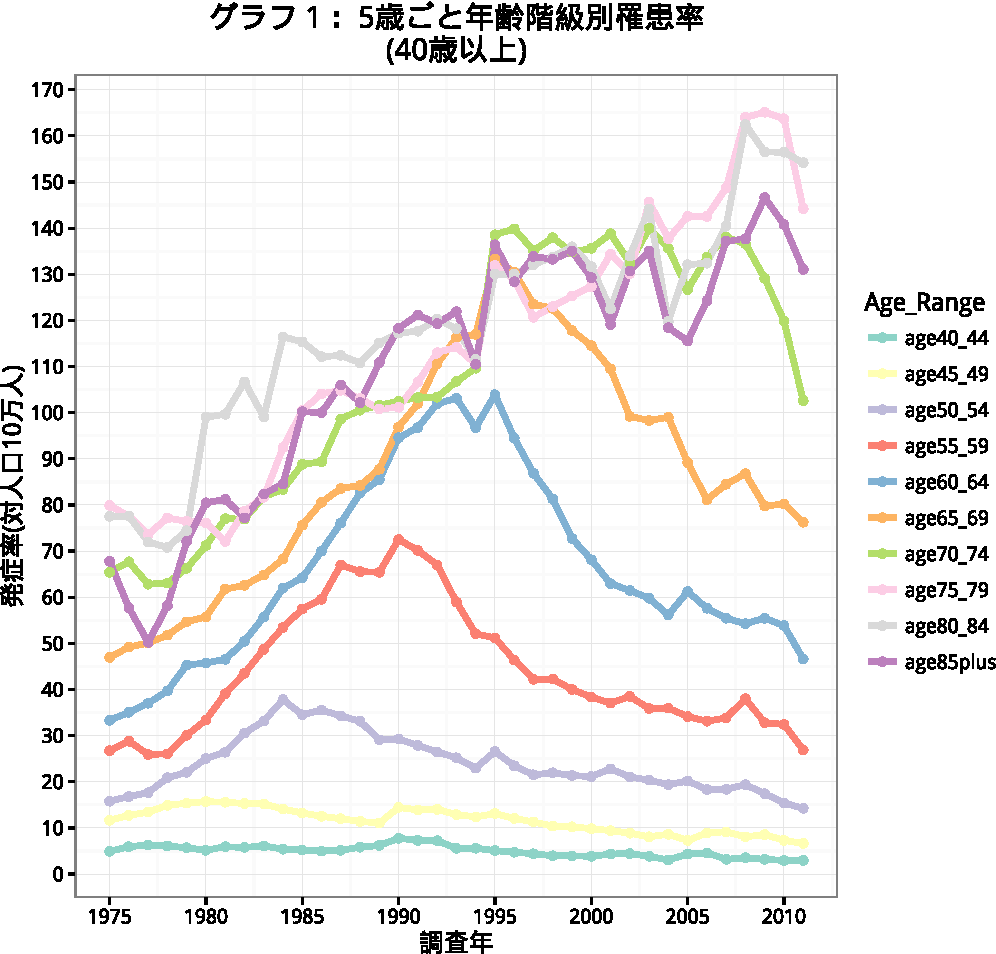
\includegraphics{example_files/figure-latex/unnamed-chunk-4-1.pdf}

\begin{Shaded}
\begin{Highlighting}[]
\CommentTok{#  グラフ2作成}

\CommentTok{# 網掛けデータ}
\NormalTok{rect <-}\StringTok{ }\KeywordTok{data.frame}\NormalTok{(}\DataTypeTok{xmin =} \DecValTok{1930}\NormalTok{, }\DataTypeTok{xmax =} \DecValTok{1935}\NormalTok{, }\DataTypeTok{ymin=}\NormalTok{-}\OtherTok{Inf}\NormalTok{, }\DataTypeTok{ymax=}\OtherTok{Inf}\NormalTok{)}

\CommentTok{#  横軸に生まれた年,診断された年齢(Age_Range)により可視化}

\KeywordTok{ggplot}\NormalTok{(}\DataTypeTok{data =} \NormalTok{rate.hepatic.melt}\FloatTok{.40}\NormalTok{,}
       \DataTypeTok{mapping =} \KeywordTok{aes}\NormalTok{(}\DataTypeTok{x =} \NormalTok{Birth_yr, }\DataTypeTok{y =} \NormalTok{Incidence_Rate,}
                     \DataTypeTok{color =} \NormalTok{Age_Range)) +}\StringTok{ }
\StringTok{  }\KeywordTok{geom_line}\NormalTok{(}\DataTypeTok{size =} \FloatTok{1.3}\NormalTok{) +}
\StringTok{  }\KeywordTok{geom_point}\NormalTok{() +}
\StringTok{    }\KeywordTok{xlab}\NormalTok{(}\StringTok{"出生年"}\NormalTok{) +}\StringTok{ }
\StringTok{    }\KeywordTok{ylab}\NormalTok{(}\StringTok{"発症率(対人口10万人)"}\NormalTok{) +}\StringTok{ }
\StringTok{    }\KeywordTok{labs}\NormalTok{(}\DataTypeTok{title =} 
           \StringTok{"グラフ2:出生年・年齢別肝がん罹患率}\CharTok{\textbackslash{}n}\StringTok{(40歳以上)"}\NormalTok{) +}\StringTok{ }
\StringTok{    }\KeywordTok{theme_bw}\NormalTok{() +}
\StringTok{    }\KeywordTok{theme}\NormalTok{(}\DataTypeTok{legend.key =} \KeywordTok{element_blank}\NormalTok{(),}
          \DataTypeTok{axis.text.x =} \KeywordTok{element_text}\NormalTok{(}\DataTypeTok{angle=}\NormalTok{-}\DecValTok{10}\NormalTok{, }\DataTypeTok{vjust=}\DecValTok{1}\NormalTok{)) +}\StringTok{ }
\StringTok{  }\KeywordTok{scale_y_continuous}\NormalTok{(}\DataTypeTok{breaks =} \KeywordTok{seq}\NormalTok{(}\DecValTok{0}\NormalTok{,}\DecValTok{170}\NormalTok{, }\DecValTok{10}\NormalTok{)) +}\StringTok{ }
\StringTok{  }\KeywordTok{scale_x_continuous}\NormalTok{(}\DataTypeTok{breaks =} \KeywordTok{seq}\NormalTok{(}\DecValTok{1890}\NormalTok{, }\DecValTok{2020}\NormalTok{, }\DecValTok{5}\NormalTok{)) +}
\StringTok{  }\KeywordTok{scale_color_brewer}\NormalTok{(}\DataTypeTok{palette =} \StringTok{"Set3"}\NormalTok{) +}\StringTok{ }
\StringTok{  }\KeywordTok{geom_rect}\NormalTok{(}\DataTypeTok{data =} \NormalTok{rect, }\KeywordTok{aes}\NormalTok{(}\DataTypeTok{xmin=}\NormalTok{xmin, }\DataTypeTok{xmax=}\NormalTok{xmax, }\DataTypeTok{ymin=}\NormalTok{ymin, }\DataTypeTok{ymax=}\NormalTok{ymax), }
            \DataTypeTok{fill =} \StringTok{"#A2B5CD"}\NormalTok{, }\DataTypeTok{inherit.aes =} \OtherTok{FALSE}\NormalTok{, }\DataTypeTok{alpha=}\FloatTok{0.5}\NormalTok{)}
\end{Highlighting}
\end{Shaded}

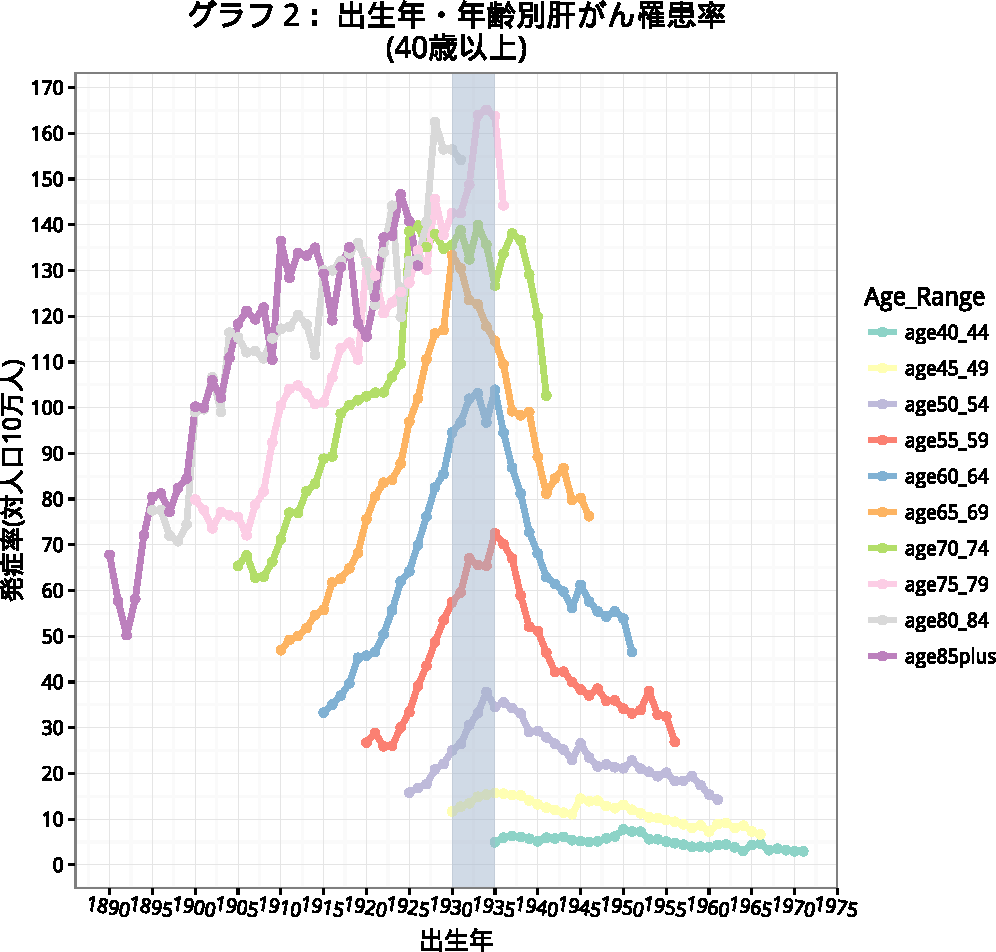
\includegraphics{example_files/figure-latex/unnamed-chunk-5-1.pdf}

\subsection{グラフ2:肝臓がんの罹患率は,1930年代前半生まれにピークがあることがわかりる(濃い網掛け).この年代生まれは,C型肝炎ウイルスの陽性割合の高い世代と一致している.}\label{1930c}

\begin{Shaded}
\begin{Highlighting}[]
\CommentTok{#  グラフ3作成}
\CommentTok{#  横軸に診断された時年齢の5歳ごと階級(Age_Range),出生コホートにより可視化}


\KeywordTok{ggplot}\NormalTok{(}\DataTypeTok{data =} \NormalTok{rate.hepatic.melt}\FloatTok{.40}\NormalTok{,}
       \DataTypeTok{mapping =} \KeywordTok{aes}\NormalTok{(}\DataTypeTok{x =} \NormalTok{Age_Range, }\DataTypeTok{y =} \NormalTok{Incidence_Rate, }\DataTypeTok{group=}\KeywordTok{factor}\NormalTok{(Birth_yr),}
                     \DataTypeTok{color =} \NormalTok{Birth_yr10)) +}\StringTok{ }
\StringTok{  }\KeywordTok{geom_line}\NormalTok{(}\DataTypeTok{size=}\FloatTok{1.3}\NormalTok{) +}
\StringTok{  }\KeywordTok{geom_point}\NormalTok{() +}
\StringTok{    }\KeywordTok{xlab}\NormalTok{(}\StringTok{"診断年齢"}\NormalTok{) +}\StringTok{ }
\StringTok{    }\KeywordTok{ylab}\NormalTok{(}\StringTok{"発症率(対人口10万人)"}\NormalTok{) +}\StringTok{ }
\StringTok{    }\KeywordTok{labs}\NormalTok{(}\DataTypeTok{title =} 
           \StringTok{"グラフ3:日本人の肝がん罹患率}\CharTok{\textbackslash{}n}\StringTok{ (出生コホートによる)"}\NormalTok{) +}\StringTok{ }
\StringTok{    }\KeywordTok{theme_bw}\NormalTok{() +}
\StringTok{    }\KeywordTok{theme}\NormalTok{(}\DataTypeTok{legend.key =} \KeywordTok{element_blank}\NormalTok{(),}
          \DataTypeTok{axis.text.x =} \KeywordTok{element_text}\NormalTok{(}\DataTypeTok{angle=}\DecValTok{10}\NormalTok{, }\DataTypeTok{vjust=}\DecValTok{1}\NormalTok{)) +}\StringTok{ }
\StringTok{  }\KeywordTok{scale_y_continuous}\NormalTok{(}\DataTypeTok{breaks =} \KeywordTok{seq}\NormalTok{(}\DecValTok{0}\NormalTok{,}\DecValTok{170}\NormalTok{, }\DecValTok{10}\NormalTok{))+}
\StringTok{  }\KeywordTok{scale_color_brewer}\NormalTok{(}\DataTypeTok{palette =} \StringTok{"Paired"}\NormalTok{)}
\end{Highlighting}
\end{Shaded}

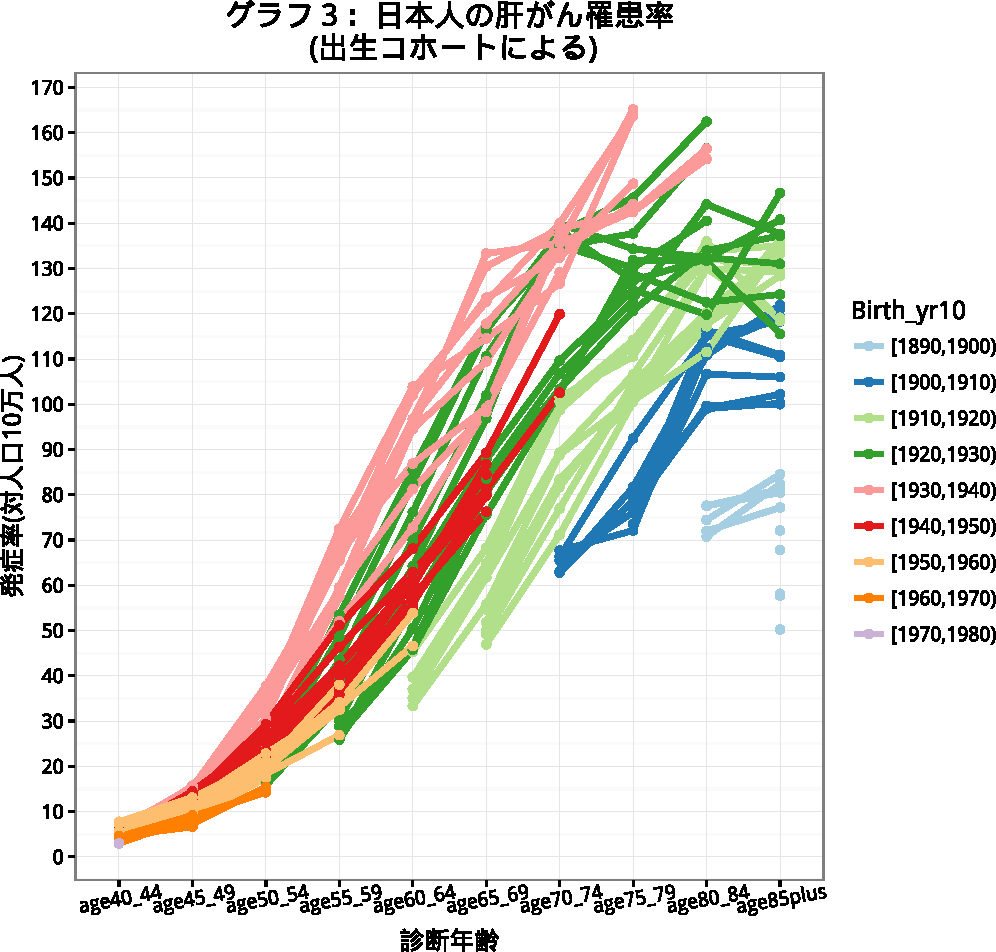
\includegraphics{example_files/figure-latex/unnamed-chunk-6-1.pdf}

\hypertarget{refs}{}

\end{document}
